\chapter{Dynamic sampling strategies for multi-domain adaptation} \label{chap:mdac}
\section{Introduction}
Building effective Neural Machine Translation models often implies accommodating diverse sets of heterogeneous data so as to optimize performance for the domain(s) of interest. Such multi-source / multi-domain adaptation problems are typically approached through instance selection or reweighting strategies, based on a static assessment of the relevance of training instances with respect to the task at hand. In this work, we study dynamic data selection strategies that are able to automatically re-evaluate the usefulness of data samples and to evolve a data selection policy in the course of training. Based on the results of multiple experiments, we show that such methods constitute a generic framework to automatically and effectively cater to a variety of real-world situations, from supervised multi-domain adaptation to unsupervised domain adaptation. 

As we usually reported in the previous chapters, MDMT train data usually admit an adverse heterogeneity in the domains' data. In the MDMT setting presented in Section ~\ref{ssec:corpora-chap4}, most common MDMT systems hardly achieve significant improvement compared to the generic model. This might prove the brittleness of the MDMT model-centric approaches to the heterogeneity of data. To overcome this challenge, we study the efficacy of the data-centric approaches, and particularly the data sampling methods.

As introduced in Chapter~\ref{chap:mdmt-review}, data sampling approaches aim to find the optimal balance of training data with respect to a certain objective, which can be one or multiple target domains. This is, however, a challenging task due, for instance, to the similarity between domains/languages, but also due to regularization effects of out-of-domain data \citep{Miceli17regularization}. It may also be suboptimal, as some target domains or languages might be easier to train than others. Finally, improving the performance of the MT system in one domain will often hurt that of another \citep{Wees17dynamic, Britz17effective}, and improving model generalization across all domains \citep{koehn18findings} may not achieve optimally for any particular domain. Several recent proposals have explored ways to instead consider \emph{dynamic} data selection and sampling strategies that surpass static strategies. Notably, \citet{Wees17dynamic,Zhang19curriculum} construct a static curriculum, while \citet{Graves17automated,Platanios19competence,Kumar19reinforcement,Wang20learning-multi,Wang20balancing} build curricula that automatically adapt to the training data.

In this chapter, we contribute to this line of research in several ways. First, we propose a novel framework (\emph{Multi-Domain Automated Curriculum}, MDAC for short) that simultaneously accounts for the domain adaptation and the multi-domain adaptation problems. Second, we propose a variant of the work of \cite{Wang20balancing} for building an automated curriculum for training Multi-Domain NMT models. We evaluate our method in various single-domain and multi-domain adaptation settings. We compare our method with several contrasts, including the work of \citet{Zhang19curriculum} and \citet{Wang20balancing}, which was previously only applied to multilingual MT. Based on these experimental results, our main conclusions are that (a) using MDAC often yields overall performance that is as good as the standard fine-tuning strategy for domain adaptation; (b) MDAC can effectively handle a variety of test situations, from targeting one single domain to the full multi-domain scenario. 

\section{Learning with multiple data sources} \label{sec:mdmt-chap7}
First, we want to recall our definition of MDMT setting in Section ~\ref{ssec:formalization-chap4}. Our train instances are distributed according to a mixture $\mathcal{D}_e^S$ such that $\mathcal{D}_e^S(x) = \sum_{d=1}^{n_d} \lambda^{s}(d) \mathcal{D}^d_e(x)$, with $\{\lambda^{s}(d), d=1 \dots n_d\}$ the mixture weights satisfying $\sum_d \lambda^{s}(d)=1$. In the sequel, we also use boldface to denote the vector $\vlambda$, and $\lambda(d)$ is used to denote a scalar corresponding to the $d^{th}$ element of the vector $\vlambda$.

The main challenge is then to make the best of this heterogeneous data, with the aim to achieve the optimal performance for the intended test conditions. These might correspond to data from just one of the training domains, as in standard supervised (multi-source) domain adaptation; a more difficult case is when the test data is from one domain unseen in training (unsupervised domain adaptation); in multi-domain adaptation finally, the test distribution is itself a mixture of domains, some of which may also be observed in training.  Without loss of generality, one may then assume that the test distribution takes the form $\mathcal{D}^{T}_e(x) = \sum_{d=1}^{n_d} \lambda^{t}(d) \mathcal{D}_e^d(x)$ - with only one non-null  component in the case of pure domain adaptation. These settings are illustrated on Figure~\ref{fig:mdmt-lambdas-chap7}.
\begin{figure}[h]
  \centering
  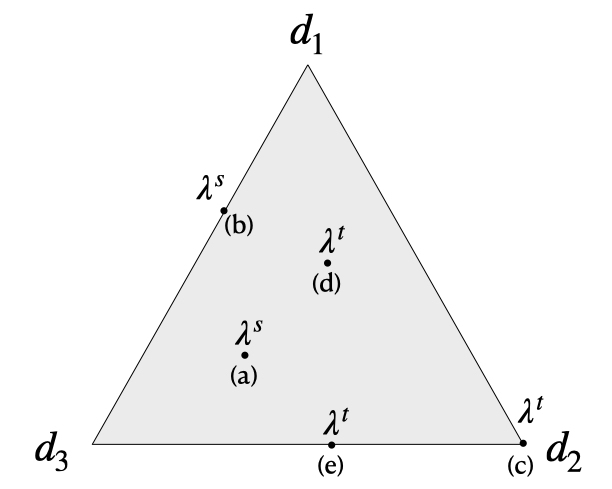
\includegraphics[width=0.48\textwidth]{graphics/mdmt-lambdas}
  \caption{Training and testing with distribution mismatch. We consider just three domains, and represent vectors of mixture weights $\vlambda^{s}$ and $\vlambda^{t}$ in the 3-dimensional simplex. Training with weights in (a) and testing with weights in (c) is supervised multi-source domain adaptation to domain~2 ($d_2$), while (b)-(c) is the unsupervised version, with no training data from $d_2$; training with weights in (a) and testing with weights in (d) is multi-domain learning, also illustrated with configurations (a)-(e) (training domain $d_1$ is not seen in test), and (b)-(d)  (test domain $d_2$ is unseen in training).}\label{fig:mdmt-lambdas-chap7}
\end{figure}

These situations have been amply documented from a theoretical perspective (eg.\ \citet{Mansour09multiple,Mansour09domain,Hoffman18algorithms}). A general recommendation in the DA setting is to adjust the sampling distribution used to optimize the system so as to compensate for the mismatch between $\mathcal{D}_e^S(x)$ and $\mathcal{D}_e^T(x)$. This can be approximated by reweighting instances, or more conveniently domains, which are selected during training with a probability $\lambda^{l}(d)$, with $\lambda^{l}(d) \neq \lambda^{s}(d)$.

A widely used approach to supervised DA is \emph{fine-tuning} \citep{Luong15stanford,Freitag16fast}, where $\vlambda^{l}$ is allowed to vary during learning. With our notations, this approach amounts to first learning an initial parameter value with all the data ($\forall d, \lambda^{l}(d) = \lambda^{s}(d)$), then to continue training with only batches from the test domain $d_t$ ($\lambda^{l}(d) = \indic{d = d_t}$) with $\indic{A}$ the indicator function for predicate $A$. Note that this strategy is potentially suboptimal, as some out-of-domain samples may contribute to the final performance due to eg.\ domain overlap. Optimizing the learning distribution in multi-domain settings is even more challenging, as the learner has to best take advantage of potential domains overlaps, and also of the fact that some domains might be easier to learn than others.

\section{Multi-Domain Automated Curriculum } \label{sec:mdac-chap7}
\subsection{Basic principles}
Assuming training data in each of the $n_d$ domains $d_1 \dots d_{n_d}$, we denote the size of the training corpus from domain $d$ as $N^{s}_d$, and $N^{s} = \sum_d N^{s}_d$ is the total number of training samples. We use $\widehat{\mathcal{D}^{d,l}_e}$ and $\widehat{\mathcal{D}^{d,t}_e}$ to denote the empirical train and test distributions for domain $d$ over the source language $e$, and $\widehat{\mathcal{D}^u_e}(x;\vlambda^{u}) = \sum_{d} \lambda^{u}(d) \widehat{\mathcal{D}^{d,u}_e}(x)$ for $u\in\{l,t\}$. In our setting,  $\vlambda^t$, and hence $\widehat{\mathcal{D}^t_e}(x;\vlambda^t)$ are fixed and predefined, approximated with an equivalent number of development corpora. 

% Our method
MDAC constructs an adaptative training distribution $\vlambda^{l}$ that optimizes the data selection policy along with the training of the NMT model. We parameterize $\vlambda^{l}$ by a differentiable function $\vlambda^l(\vpsi)$. We divide the training into many short sessions; in each session $t$, the model is trained with a static data distribution $\vlambda^{l}(\vpsi_t)$. After one learning session, we update the data distribution using the REINFORCE algorithm of \citet{Williams92simple}. The evolution of $\vpsi$ is thus defined by:
\begin{align*}
\vpsi_{t+1} &= \vpsi_t + \mathbf{lr}_{1} * \displaystyle{\mathop{\sum}_{d=1}^{n_d}} R(d) * \frac{\partial \lambda^l(d;\vpsi_t)}{\partial \vpsi}, \\
\end{align*}
\begingroup
\allowdisplaybreaks
where reward $R(d)$ is computed as:
\begin{align*}
  R(d) = J^t(\theta_t,\vlambda^t) - J^t(\theta_{t+k},\vlambda^t),
\end{align*}
and where we also define:
\begin{equation}
\begin{array}{rcl}
\theta_{t+i} &=& Update\big(\theta_{t+i-1},[x^i_j,y^i_j]_{j=1}^N\big) \\ \nonumber
x^i_j &\sim& \widehat{D^{d,l}_e}(x), y^i_j \sim g^d(x^i_j) \\
J^t(\theta,\vlambda_t) &=& \displaystyle{\mathop{\sum}_{d=1}^{n_d}}\lambda^t(d)\displaystyle{\mathop{\sum}_{x^{d,t} \sim \widehat{D^{d,t}_e},y^{d,t} \sim g^d(x^{d,t})}} l(\theta,x^{d,t},y^{d,t}).
\end{array}
\end{equation}
\endgroup

In these equations, $N$ denotes the size of a batch; $\mathbf{lr}_{1}$ is the learning rate of the sampling distribution; $l(\theta,x,y) = $ is the loss of the NMT model on sample $(x,y)$; $J^t(\theta,\vlambda_t)$ is the weighted loss aggregated over $n_d$ dev-sets corresponding to the $n_d$ domains.

To compute the reward $R(d)$ of using data from domain $d$ to train the model, we simulate $k$ training steps from the current checkpoint by training the model with $k$ batches sampled from $D^l(d)$ and compute the gain of the weighted dev-loss. This computation is inspired by the target prediction gain in \citet{Graves17automated}. However, where \citet{Graves17automated} used accumulated gains from the past as rewards, we instead predict the usefulness of each domain for improving the future performance of the system given its current state. This is achieved by simulating a round of training with only the data from one domain. Furthermore, the choice of the parameterization of the sampling distribution in our method differs from that of \citet{Graves17automated}, although this choice is empirical.

The work of \citet{Wang20balancing} is also related: it is based on the Bi-level Optimization framework, which aims to find an optimal static distribution $\vlambda^{l}$ that will result in the best NMT model with respect to a given target dev set at the end of training. These authors also derive a similar form of update for $\vpsi$. However, their reward is the cosine similarity between the gradient computed with the training data from one domain and the gradient computed with the dev set. We compare this approach with ours in the experiment section.

\subsection{MDAC for (multi) domain adaptation}
The setting developed in previous sections is quite general and can, in principle, accommodate the variety of situations mentioned above, and many more: basic domain adaption, multi-domain adaptation with various target distributions, possibly including domains unseen in training. In our experiments, we would like to better assess the true potential of MDAC in these settings and seek to experimentally answer the following questions:
\begin{itemize}
\item is MDAC a viable alternative to conventional fine-tuning? In particular, does it enable to better take advantage of relevant data from other domains?
\item is MDAC also a viable option in multi-domain adaptation scenarios?
\item does MDAC also enable to perform \emph{unsupervised} (multi-)domain adaptation? \fyDone{TBContinued}
\end{itemize}
These questions are further explored in section~\ref{sec:results-chap7}. We now turn to our experimental conditions.

\section{Experimental settings} \label{sec:exp-chap7}
\subsection{Data and metrics \label{ssec:corpora-chap7}}
In this work, we reuse the MDMT setting of Section ~\ref{ssec:corpora-chap4}, which has proved to be challenging for MDMT systems. We uses the same metric and processing procedure as in Section ~\ref{ssec:corpora-chap4}. For the sake of brevity, we will not provide the description here.

\subsection{Baseline systems \label{ssec:baseline-chap7}}
Our baselines are standard for multi-domain systems.\footnote{We however omit domain-specific systems trained only with the corresponding subset of the data, which are always inferior to the mix-domain strategy \citep{Britz17effective}.} Using Transformers \citep{Vaswani17attention} implemented in OpenNMT-tf\footnote{\url{https://github.com/OpenNMT/OpenNMT-tf}} \citep{Klein17opennmt}, we build the following systems:

\begin{itemize}
\itemsep0em 
\item Generic models trained with predefined mixtures of the training data taking the form:
\begin{align} \label{mixture:trn-chap7}
\lambda_{\alpha}(d) = \frac{q_d^{\alpha}}{\displaystyle{\mathop{\sum}_{d=1}^{n_d}q_d^{\alpha}}} &&
q_d = \frac{\mid N^{s}_d \mid}{\displaystyle{N^{s}}} % \mathop{\sum}_{i=1}^K\mid D_i \mid}}
\end{align}
with $\alpha \in \{0,0.25,0.5,0.75,1.0\}$. We denote these as \system{Mixed-$\alpha$} below. \system{Mixed-$0$} uses a uniform distribution, \system{Mixed-$1.0$} the empirical domain distribution;
\item fine-tuned models \citep{Luong15stanford,Freitag16fast} which was already presented in Section ~\ref{ssec:baselines-chap4}. Their implementations are provided in Appendix ~\ref{appendix:a};
\item systems trained with fixed data mixtures corresponding to $\vlambda^l \in \big[ \vlambda_0, \vlambda_{0.25}, \vlambda_{0.5}, \vlambda_{0.75}, \vlambda_{1.0}\big]$; these are used in the multi-domain experiments of Section~\ref{ssec:mda-chap7};
\item  our own implementations of recent dynamic sampling proposals from the literature: Curriculum Learning (CL) of \citet{Zhang19curriculum} and Differential Data Selection (DDS) of \citet{Wang20balancing} (see details below);
\end{itemize}

All models use embeddings and hidden layers of dimension~512. Transformer models contain 8~attention heads in each of the 6+6 layers; the inner feedforward layer contains 2048 cells. Training lasts for 200K iterations, with batches of~12,288 tokens, Adam with parameters $\beta_1=0.9$, $\beta_2= 0.98$, Noam decay ($warmup\_steps=4000$), and a dropout rate of $0.1$ in all layers.

\subsection{CL and DDS's re-implementation}\fyDone{Right place for this ?}
We re-implement DDS in Tensorflow without any change in the choices of parameterization and hyper-parameters compared to the original code of \citet{Wang20balancing}.\footnote{\url{https://github.com/cindyxinyiwang/multiDDS}}
% 
We also re-implement the approach of \citet{Zhang19curriculum} according to the authors' description. For each domain adaptation experiment, we combine the training data of all other domains into one corpus then compute the cross-entropy difference score of each source sentence of this combined dataset. We then sort and split the corpus into 9 shards and execute curriculum learning with 10 shards, using the in-domain corpus as the first shard.

\subsection{MDAC systems} \label{ssec:dds-sys-chap7}
The behavior of MDAC only depends on (a) the initial domain distribution at the start of training $\vlambda^{l}_{t=0}$, and (b) the targeted (dev/test) distribution $\vlambda^{t}$. We thus report these systems as \system{MDAC($\vlambda^{l}_{t=0}$, $\vlambda^{t}$)} and compare with DDS using the same settings.

In our work, we parameterize the distribution $\vlambda^l$ as follows (with $\beta=2$\footnote{This setting corresponds to the \emph{spherical softmax} of \cite{Brebisson16anexploration}.} in all experiments):\fyDone{Explain why}
\begin{equation}
\lambda^l(d;\vpsi) = \frac{\psi[d]^\beta}{\sum_i \psi[i]^\beta}. \nonumber
\end{equation}
This parameterization avoids the ``rich-get-richer'' effect that we observe when using $\vlambda(\vpsi) = \operatorname{softmax}(\vpsi)$, which yields gradients wrt. $\psi[d]$ that are proportional to $\exp(\psi[d])$ (see also Figure~\ref{fig:sampling-chap7}). Additional settings for the hyper-parameters of our method include the number of simulation steps $k=10$ and the learning rate $\mathbf{lr}_{data}=0.001$. We update the sampling distribution via 100 gradient descent iterations for almost all experimental settings except that for adaptation with automatic clusters (Section~\ref{ssec:clda-chap7}), where we use 20~gradient descent iterations to avoid converging to degenerate distributions.\fyFuture{Why? computation?} We split the training into 100 short sessions that last 2000 training steps each. The choice of those hyper-parameters is mostly heuristic except for the learning rate $\mathbf{lr}_{data}$ which is optimized via grid search over a set of values $\{0.001,0.0025,0.005\}$.

The computational cost of our approach is due to the simulation step, which is conducted after every 2000 iterations to compute the reward of each domain. During the simulation step, we update the temporary checkpoint with $k$ updates for each domain, which cost as much as $k$ training updates. Therefore, we execute $k \times n_d$ updates in total after every 2000 iterations. Our algorithm approximately costs $1 + \frac{k \times n_d}{2000}$ times as much as a standard training.

\subsection{Experimental tasks}
We evaluate and compare our method with multiple baselines in the 5 following conditions.
%including: domain adaptation; multi-domain adaptation, bi-domain adaptation, unseen domain adaptation, and unsupervised domain adaptation.
In the \emph{supervised domain adaptation task}, given the data from 6 domains (\domain{med}, \domain{bank}, \domain{law}, \domain{it}, \domain{talk}, \domain{rel}), we aim to build distinct expert NMT models for each domain. To challenge the flexibility of the method, we also consider a \emph{bi-domain adaptation task}, where given the same 6 domains, we only focus on adapating only to 2 domains.

In the \emph{multi-domain adaptation task}, given the same 6 domains, we aim to build one single NMT model that would perform optimally, assuming a uniform distribution of domains during the test.

In a fourth experiment (\emph{unseen domain adaptation}), given training data in 6 domains and a small development set of a new domain (\domain{News} in our case), we aim to build an NMT model which performs well for the unseen domain.

Finally, in the \emph{unsupervised domain adaptation task}, we cluster all available training data into 30~clusters using the KNN algorithm in the same way as in \citep{Tars18multidomain}, then adapt these clusters to one of 6 domains using the corresponding in-domain dev set. We compare MDAC to DDS for each of our 6 test sets.

\section{Results and discussion \label{sec:results-chap7}}
\subsection{Domain Adaptation}\label{ssec:da-chap7}
In this setting, we aim to build an NMT model for one single domain: we accordingly set $\vlambda^t$ to a deterministic distribution $\vlambda_d$, where the target domain $d$ has probability~1.

We consider three initializations for MDAC and DDS, using $\vlambda_0$, $\vlambda_1$ and $\vlambda_d$. According to Table~\ref{tab:da-chap7}, MDAC achieves the overall best performance when $\vlambda_{t=0} = \vlambda_0$.  Doing so proves much better than initializing with $\vlambda_d$ for small domains: \domain{talk}, \domain{bank} and\domain{it}. Conversely, initializing with $\vlambda_d$ is beneficial when targeting large domains such as \domain{med} and \domain{law}. The same conclusion holds for DDS. 

We now compare the best MDAC system (using $\vlambda_{t=0} = \vlambda_0$) to full fine-tuning. According to Table~\ref{tab:da-chap7}, fine-tuning is better for large domains such as \domain{med} and \domain{law}, while MDAC outperforms fine-tuning by approximately 1.2 BLEU for \domain{bank} and 1.0 BLEU for \domain{rel}. This indicates that for small domains, out-of-domain data helps improve the generalization and that MDAC is able to exploit both the in-domain and the out-of-domain training data instead of edging out the out-of-domain training data as in fine-tuning. Results for DDS display similar trends but are always outperformed by MDAC. The behavior of CL, which does only well the large domain \domain{med} lag somewhat behind.

\begin{table*}[htbp]
  \centering \small
  \begin{tabular}{|l|*8{r|}} \hline
    domain \hfill $d=$ & \multicolumn{1}{c|}{\domain{ med}} & \multicolumn{1}{c|}{\domain{ law}} & \multicolumn{1}{c|}{\domain{bank}} & \multicolumn{1}{c|}{\domain{talk}} & \multicolumn{1}{c|}{\domain{ it }} & \multicolumn{1}{c|}{\domain{ rel}} & \multicolumn{1}{c|}{avg.} \\ \hline
    FT-Full($d$) &40.3&63.8&54.4&38.5&52.0&91.0&56.7\\ \hline
    \hline
    \system{CL($d$)} &40.2&60.2&53.7&36.5&51.1&91.1&55.5\\ \hline
    \system{DDS($\vlambda_0, \vlambda_d$)} &39.6&60.1&55.0&38.5&52.5&92.0&56.3\\
    \system{MDAC($\vlambda_0, \vlambda_d$)} &39.6&62.5$^{**}$&55.6$^{*}$&38.5&52.4&92$^{***}$&56.8\\
     \hline
    \system{DDS($\vlambda_1, \vlambda_d$)} &39.7&53.9&49.6&37.9&43.1&64.3&48.1\\
    \system{MDAC($\vlambda_1, \vlambda_d$)} &40.2&59.9&52.6&38.5&50.7&79.8&53.6\\ \hline
    \system{DDS($\vlambda_d, \vlambda_d$)} &39.9&63.9&54.5&35.4&51.2&91.8&56.1\\
    \system{MDAC($\vlambda_d, \vlambda_d$)}&40.6&63.9&54.5&35.6&51.3&92.3&56.4\\
    \hline
  \end{tabular}
  \caption{Domain adaptation experiments. We report BLEU scores of each method for 6 target domains and their average: each column corresponds to a distinct system. ($^{*}$) MDAC is significantly better than CL, fine-tuning and DDS with $p<0.05$. ($^{**}$) MDAC is significantly better than CL and DDS with $p<0.05$. ($^{***}$) MDAC is significantly better than CL, fine-tuning with $p<0.05$.}
  \label{tab:da-chap7}
\end{table*}

\subsection{Bi-domain adaptation}\label{ssec:bida-chap7}

In these control experiments, we showcase the flexibility of dynamic sampling and try to adapt to (arbitrary) pairs of target domains with equal weight and contrast our results with those of DDS. Results are in Table~\ref{tab:bi-da-chap7}. Here, MDAC significantly outperforms DDS in two settings (\domain{med+it} and \domain{law+bank}) while being surpassed in \domain{talk+rel}.
% Allthough we showing that MDAC is capable to adapt to a variable set of target domains.

\subsection{Multi-domain adaptation}\label{ssec:mda-chap7}

We now turn to a more realistic scenario and consider multi-domain adaptation, which aims to train one single system with optimal performance averaged over 6 domains. This setting targets a uniform test distribution $\vlambda^t = \vlambda_0$. In this situation, CL \citep{Zhang19curriculum} does not apply. We therefore only contrast the performance of MDAC, DDS and several fixed training data distribution $\vlambda^l \in \big[ \vlambda_0, \vlambda_{0.25}, \vlambda_{0.5}, \vlambda_{0.75}, \vlambda_{1.0}\big]$, where $\vlambda_{\alpha}$ is defined according to equation~\eqref{mixture:trn-chap7}.

We again initialize MDAC and DDS with two distribution $\vlambda_0$ and $\vlambda_1$. According to Table~\ref{tab:multi-da-chap7}, MDAC achieves the best performance with initial (uniform) $\vlambda_0$. The same conclusion holds for DDS. For this configuration, MDAC outperforms in average static training distributions including $\big[ \vlambda_0, \vlambda_{0.75}, \vlambda_{1.0}\big]$ by a significant margin, and performs slightly better than $\big[ \vlambda_{0.25}, \vlambda_{0.5} \big]$. This indicates that MDAC allows us to skip the somewhat heuristic choice of the optimal training mixture.

A second observation is that DDS is again outperformed by MDAC by a significant margin of 1.5 BLEU on average; the only domain where DDS does (much) better is \domain{med}. Figure~\ref{fig:sampling-chap7}, where we plot the evolution of the training mixture in the course of training sessions, helps understand the difference between the two methods. For DDS (Figure~\ref{fig:DDS-chap7}), the sampling distribution quickly converges towards a bi-domain mode in which only \domain{med} and \domain{rel} have significant probability -- hence the good performance on the former domain. In contrast, the distribution computed by MDAC evolves more smoothly; small domains such as \domain{bank}, \domain{it}, \domain{talk} and \domain{rel} receive a larger proportion of training data in the early stages; their weights then slowly decrease as larger domains such as \domain{med} and \domain{law} increase their share. This, however, only happens at the end of the training, when the NMT models might have already been close to their optimal performance for the small domains.

\begin{table*}[htbp]
  \centering \small
  \begin{tabular}{|l|*7{r|}} \hline
    domain \hfill $d=$ & \multicolumn{1}{c|}{\domain{ med}} & \multicolumn{1}{c|}{\domain{ law}} & \multicolumn{1}{c|}{\domain{bank}} & \multicolumn{1}{c|}{\domain{talk}} & \multicolumn{1}{c|}{\domain{ it }} & \multicolumn{1}{c|}{\domain{ rel}} \\ \hline \hline
    \system{DDS($\vlambda_0, \vlambda_2$)}&39.5&-&-&-&50.1&- \\
    \system{MDAC($\vlambda_0, \vlambda_2$)}&39.1&-&-&-&51.8$^*$&- \\
    \system{DDS($\vlambda_0, \vlambda_2$)}&-&60.8&53.3&-&-&- \\
    \system{MDAC($\vlambda_0, \vlambda_2$)}&-&61.9$^*$&54.5$^*$&-&-&- \\
    \system{DDS($\vlambda_0, \vlambda_2$)}&-&-&-&37.9&-&91.3 \\ 
    \system{MDAC($\vlambda_0, \vlambda_2$)}&-&-&-&36.9&-&90.4 \\
    \hline
  \end{tabular}
  \caption{Adapting to two domains. For a given line, non empty columns correspond to the pair of target domains. ($^*$) MDAC is significantly better than DDS with $p<0.05$.}
  \label{tab:bi-da-chap7}
\end{table*}

\begin{table*}[htbp]
  \centering \small
  \begin{tabular}{|l|*8{r|}} \hline
    domain \hfill $d=$ & \multicolumn{1}{c|}{\domain{ med}} & \multicolumn{1}{c|}{\domain{ law}} & \multicolumn{1}{c|}{\domain{bank}} & \multicolumn{1}{c|}{\domain{talk}} & \multicolumn{1}{c|}{\domain{ it }} & \multicolumn{1}{c|}{\domain{ rel}} & \multicolumn{1}{c|}{mean} \\ \hline \hline
    % Multidomain
    \system{Mixed-0} &38.6&59.3&53.7&37.3&51.0&90.4&55.1\\
    \system{Mixed-0.25}&38.9&59.6&53.3&37.6&50.5&90.6&55.1\\
    \system{Mixed-0.5}&39.0&60.2&52.5&38.5&51.9&90.3&55.4\\
    \system{Mixed-0.75}&39.4&59.9&51.9&38.8&50.0&87.6&54.6\\
    \system{Mixed-1}&40.3&59.5&49.8&36.4&49.0&80.0&52.5\\
    \hline \hline
    \system{DDS($\vlambda_0, \vlambda_0$)} &40.1&56.9&50.7&37.4&46.8&92.0&54.0\\ 
    \system{MDAC($\vlambda_0, \vlambda_0$)}&38.5&60.3$^{**}$&54.4$^*$&37.3&51.3$^{**}$&91.4$^*$&55.5$^{**}$\\ 
    \hline \hline
    \system{DDS($\vlambda_1, \vlambda_0$)} &40.6&55.5&48.0&36.2&46.9&60.1&47.9\\
    \system{MDAC($\vlambda_1, \vlambda_0$)}&40.2&59.3$^{**}$&51.0$^{**}$&36.9$^{**}$&48.6$^{**}$&80.7$^{**}$&52.8$^{**}$\\
    \hline
  \end{tabular}
  \caption{Multi domain adaptation. For a given line, all the columns \emph{correspond to the same multi-domain system}. ($^*$) MDAC is significantly better than \system{Mixed-$\alpha$} with $p<0.05$. ($^{**}$) MDAC is significantly better than DDS with $p<0.05$.}
  \label{tab:multi-da-chap7}
\end{table*}

\begin{figure*}[htbp]
\begin{subfigure}{.5\textwidth}
  \centering
  % include first image
  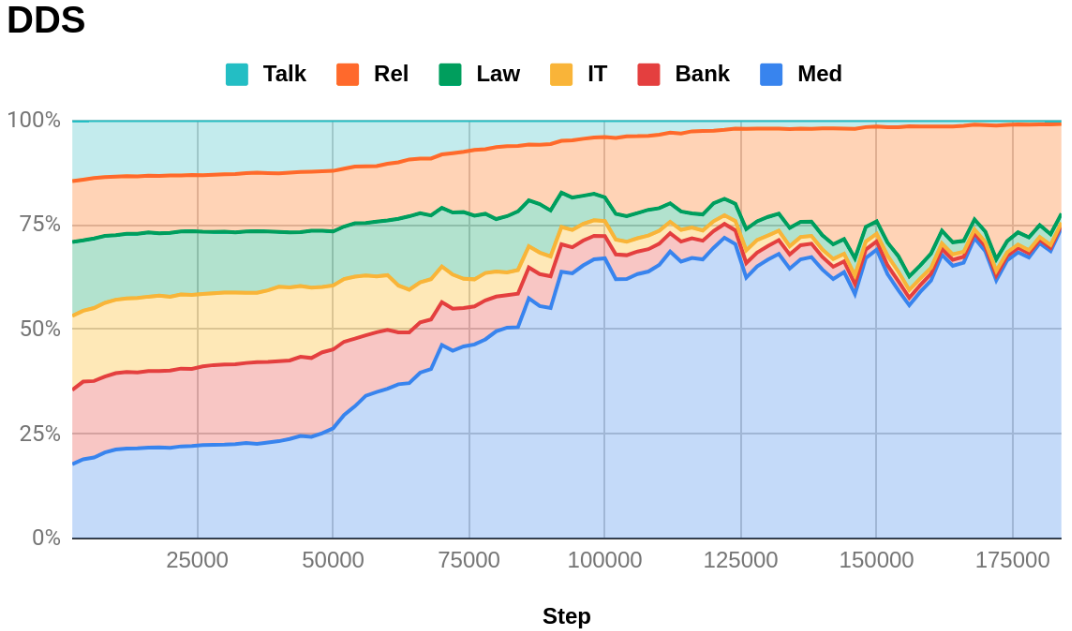
\includegraphics[width=0.97\textwidth]{graphics/DDS.png}  
  \caption{DDS}
  \label{fig:DDS-chap7}
\end{subfigure}
\begin{subfigure}{.5\textwidth}
  \centering
  % include second image
  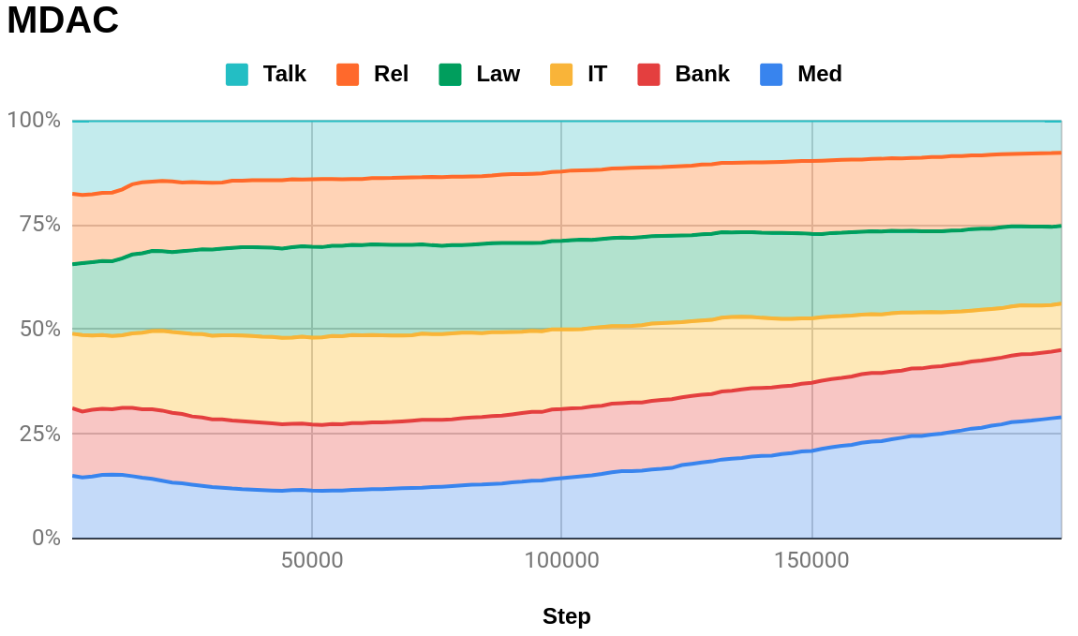
\includegraphics[width=0.97\textwidth]{graphics/MDAC.png}  
  \caption{MDAC}
  \label{fig:MDAC-chap7}
\end{subfigure}
\caption{Evolution of the sampling distribution during training.}
\label{fig:sampling-chap7}
\end{figure*}

\begin{table*}[htbp]
  \centering \small
  \begin{tabular}{|l|*{10}{r|}} \cline{1-2} \cline{4-11}
    domain \hfill $d=$ & \multicolumn{1}{c|}{\domain{news}}& \hfill &domain \hfill $d=$ & \multicolumn{1}{c|}{\domain{ med}} & \multicolumn{1}{c|}{\domain{ law}} & \multicolumn{1}{c|}{\domain{bank}} & \multicolumn{1}{c|}{\domain{talk}} & \multicolumn{1}{c|}{\domain{ it }} & \multicolumn{1}{c|}{\domain{ rel}} & \multicolumn{1}{c|}{mean}  \\ 
\cline{1-2} \cline{4-11}
    \multicolumn{2}{|c|}{\sl Unseen domain} & &\multicolumn{8}{c|}{\sl Training with 30 clusters} \\ 
\cline{1-2} \cline{4-11}
    \system{Mixed-0}      & 25.7 & &\system{DDS($\vlambda^*, \vlambda_d$)}&38.3&60.1&50.3&35.8&49.1&90.1&53.9\\
    \system{Mixed-0.25} & 25.8 & &\system{MDAC($\vlambda^*, \vlambda_d$)}&39.2$^*$&61.6$^*$&52.0$^*$&38.2$^*$&49.1&89.7&55.0$^*$\\ \cline{4-11}
    \system{Mixed-0.5}   &26.5\\
    \system{Mixed-0.75} &26.8\\
    \system{Mixed-1} &26.9 \\
    \cline{1-2}
     \system{DDS($\vlambda_0, \vlambda_{news}$)} &26.3 \\
     \system{MDAC($\vlambda_0, \vlambda_{news}$)} &26.3 \\
     \cline{1-2}
  \end{tabular}
  \caption{Unseen domain adaptation (left) and unsupervised adaptation (right). For a given line, each column corresponds to one distinct system. ($^*$) MDAC is significantly better than DDS.}
  \label{tab:unsupervised-da-chap7}
\end{table*}

\subsection{Unseen domain}\label{ssec:uda-chap7}
The left part of Table~\ref{tab:unsupervised-da-chap7} displays the performance on the unseen domain \domain{news} for NMT systems trained with the mixtures $\vlambda^l \in \big[ \vlambda_0, \vlambda_{0.25}, \vlambda_{0.5}, \vlambda_{0.75}, \vlambda_{1.0}\big]$ and with dynamic data selection (MDAC and DDS). These systems have insignificant differences in BLEU, showing that dynamic mixture does not improve the robustness of the NMT system against unseen domains. However, the fact that the performance of MDAC and DDS is close to the best performance is a sign that they can also apply in such challenging situations. % the robustness of the NMT model.

\subsection{Automatic clustering}\label{ssec:clda-chap7}
The right part of Table~\ref{tab:unsupervised-da-chap7} reports the performance of NMT systems adapted to each domain.\footnote{A more detailed analysis is in the supplementary material.} In comparison to Section~\ref{ssec:da-chap7}, the training data is distributed in 30 automatic clusters instead of the 6 original domains. Splitting the train data into small groups provides the learner with extra degrees of freedom when selecting the best distribution. However, as these clusters are built automatically, they are noisier in nature. According to the results in Table~\ref{tab:unsupervised-da-chap7}, this scenario is hard both for DDS and MDAC, which perform much worse than for the supervised DA setting. This again signals the importance of initialization: analyzing the clustering, we find that the data for \domain{rel} mostly correspond to one single cluster. When using a uniform initialization, this cluster starts with a very small weight and never succeeds in yielding the (good) performance observed in the DA setting.

\subsection{Reward analysis}

\begin{figure*}[htbp]
\begin{subfigure}{.5\textwidth}
  \centering
  % include first image
  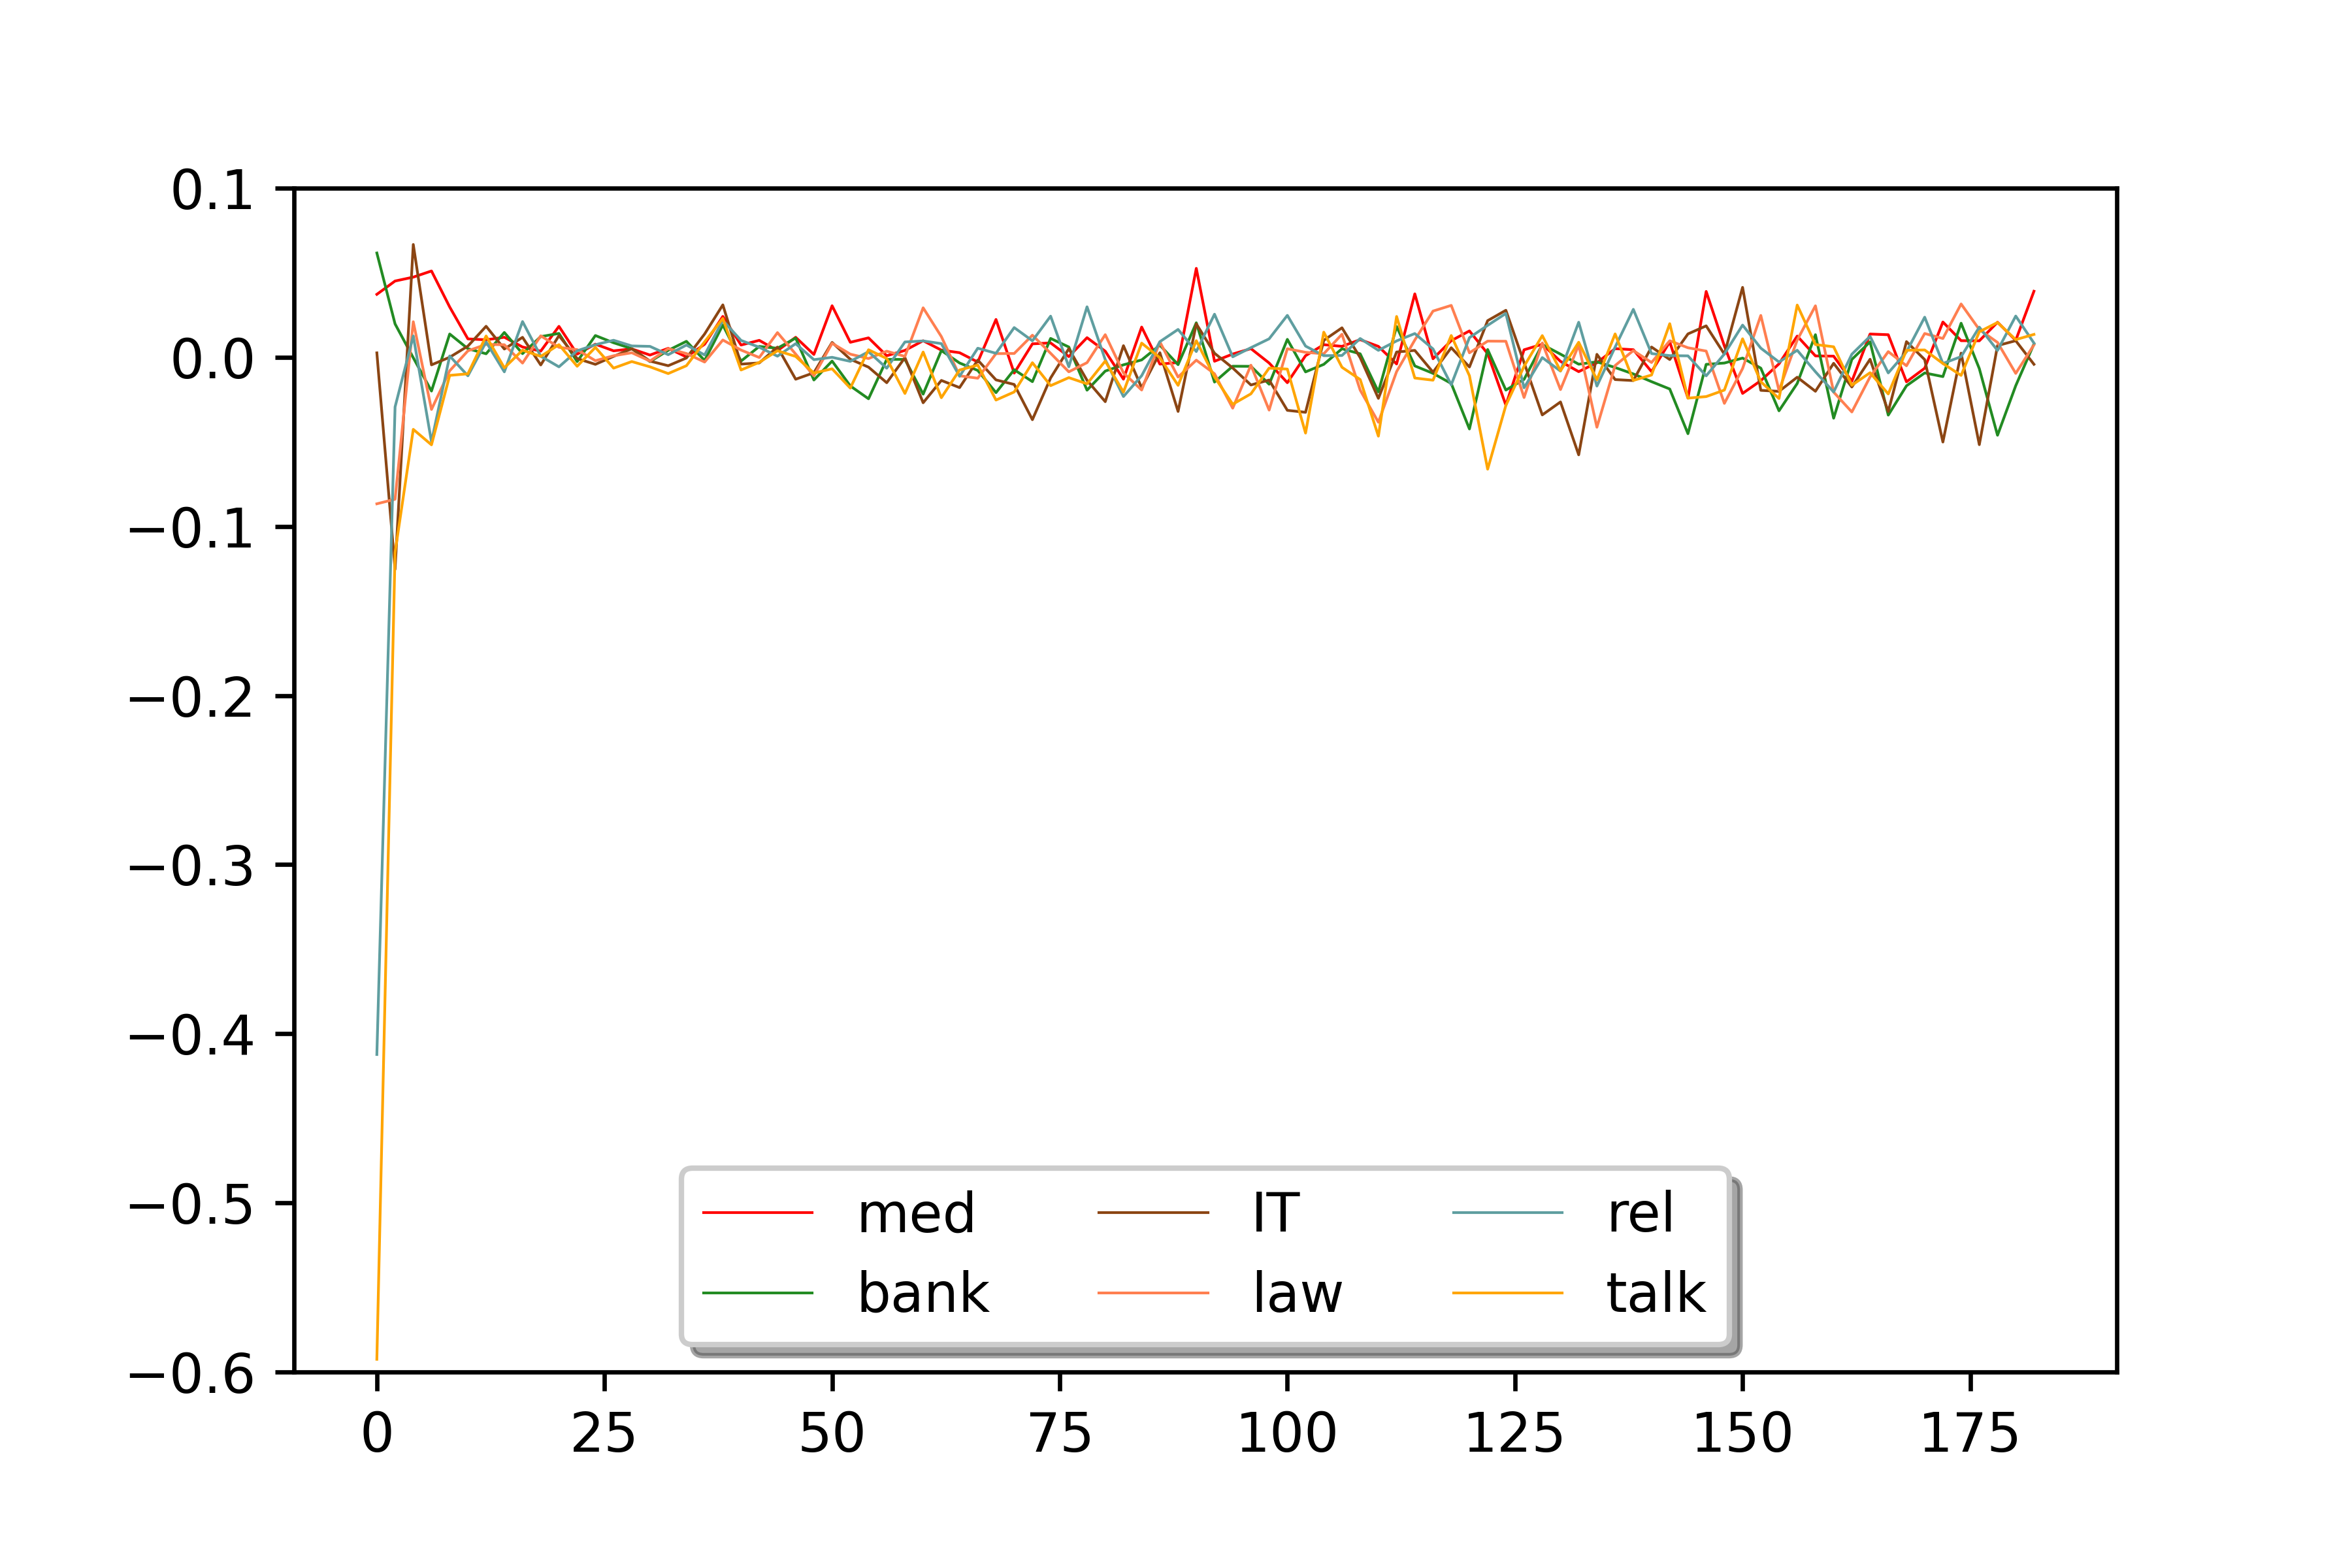
\includegraphics[width=0.97\textwidth]{graphics/rewards_dds.png}  
  \caption{DDS}
  \label{fig:reward-dds-chap7}
\end{subfigure}
\begin{subfigure}{.5\textwidth}
  \centering
  % include second image
  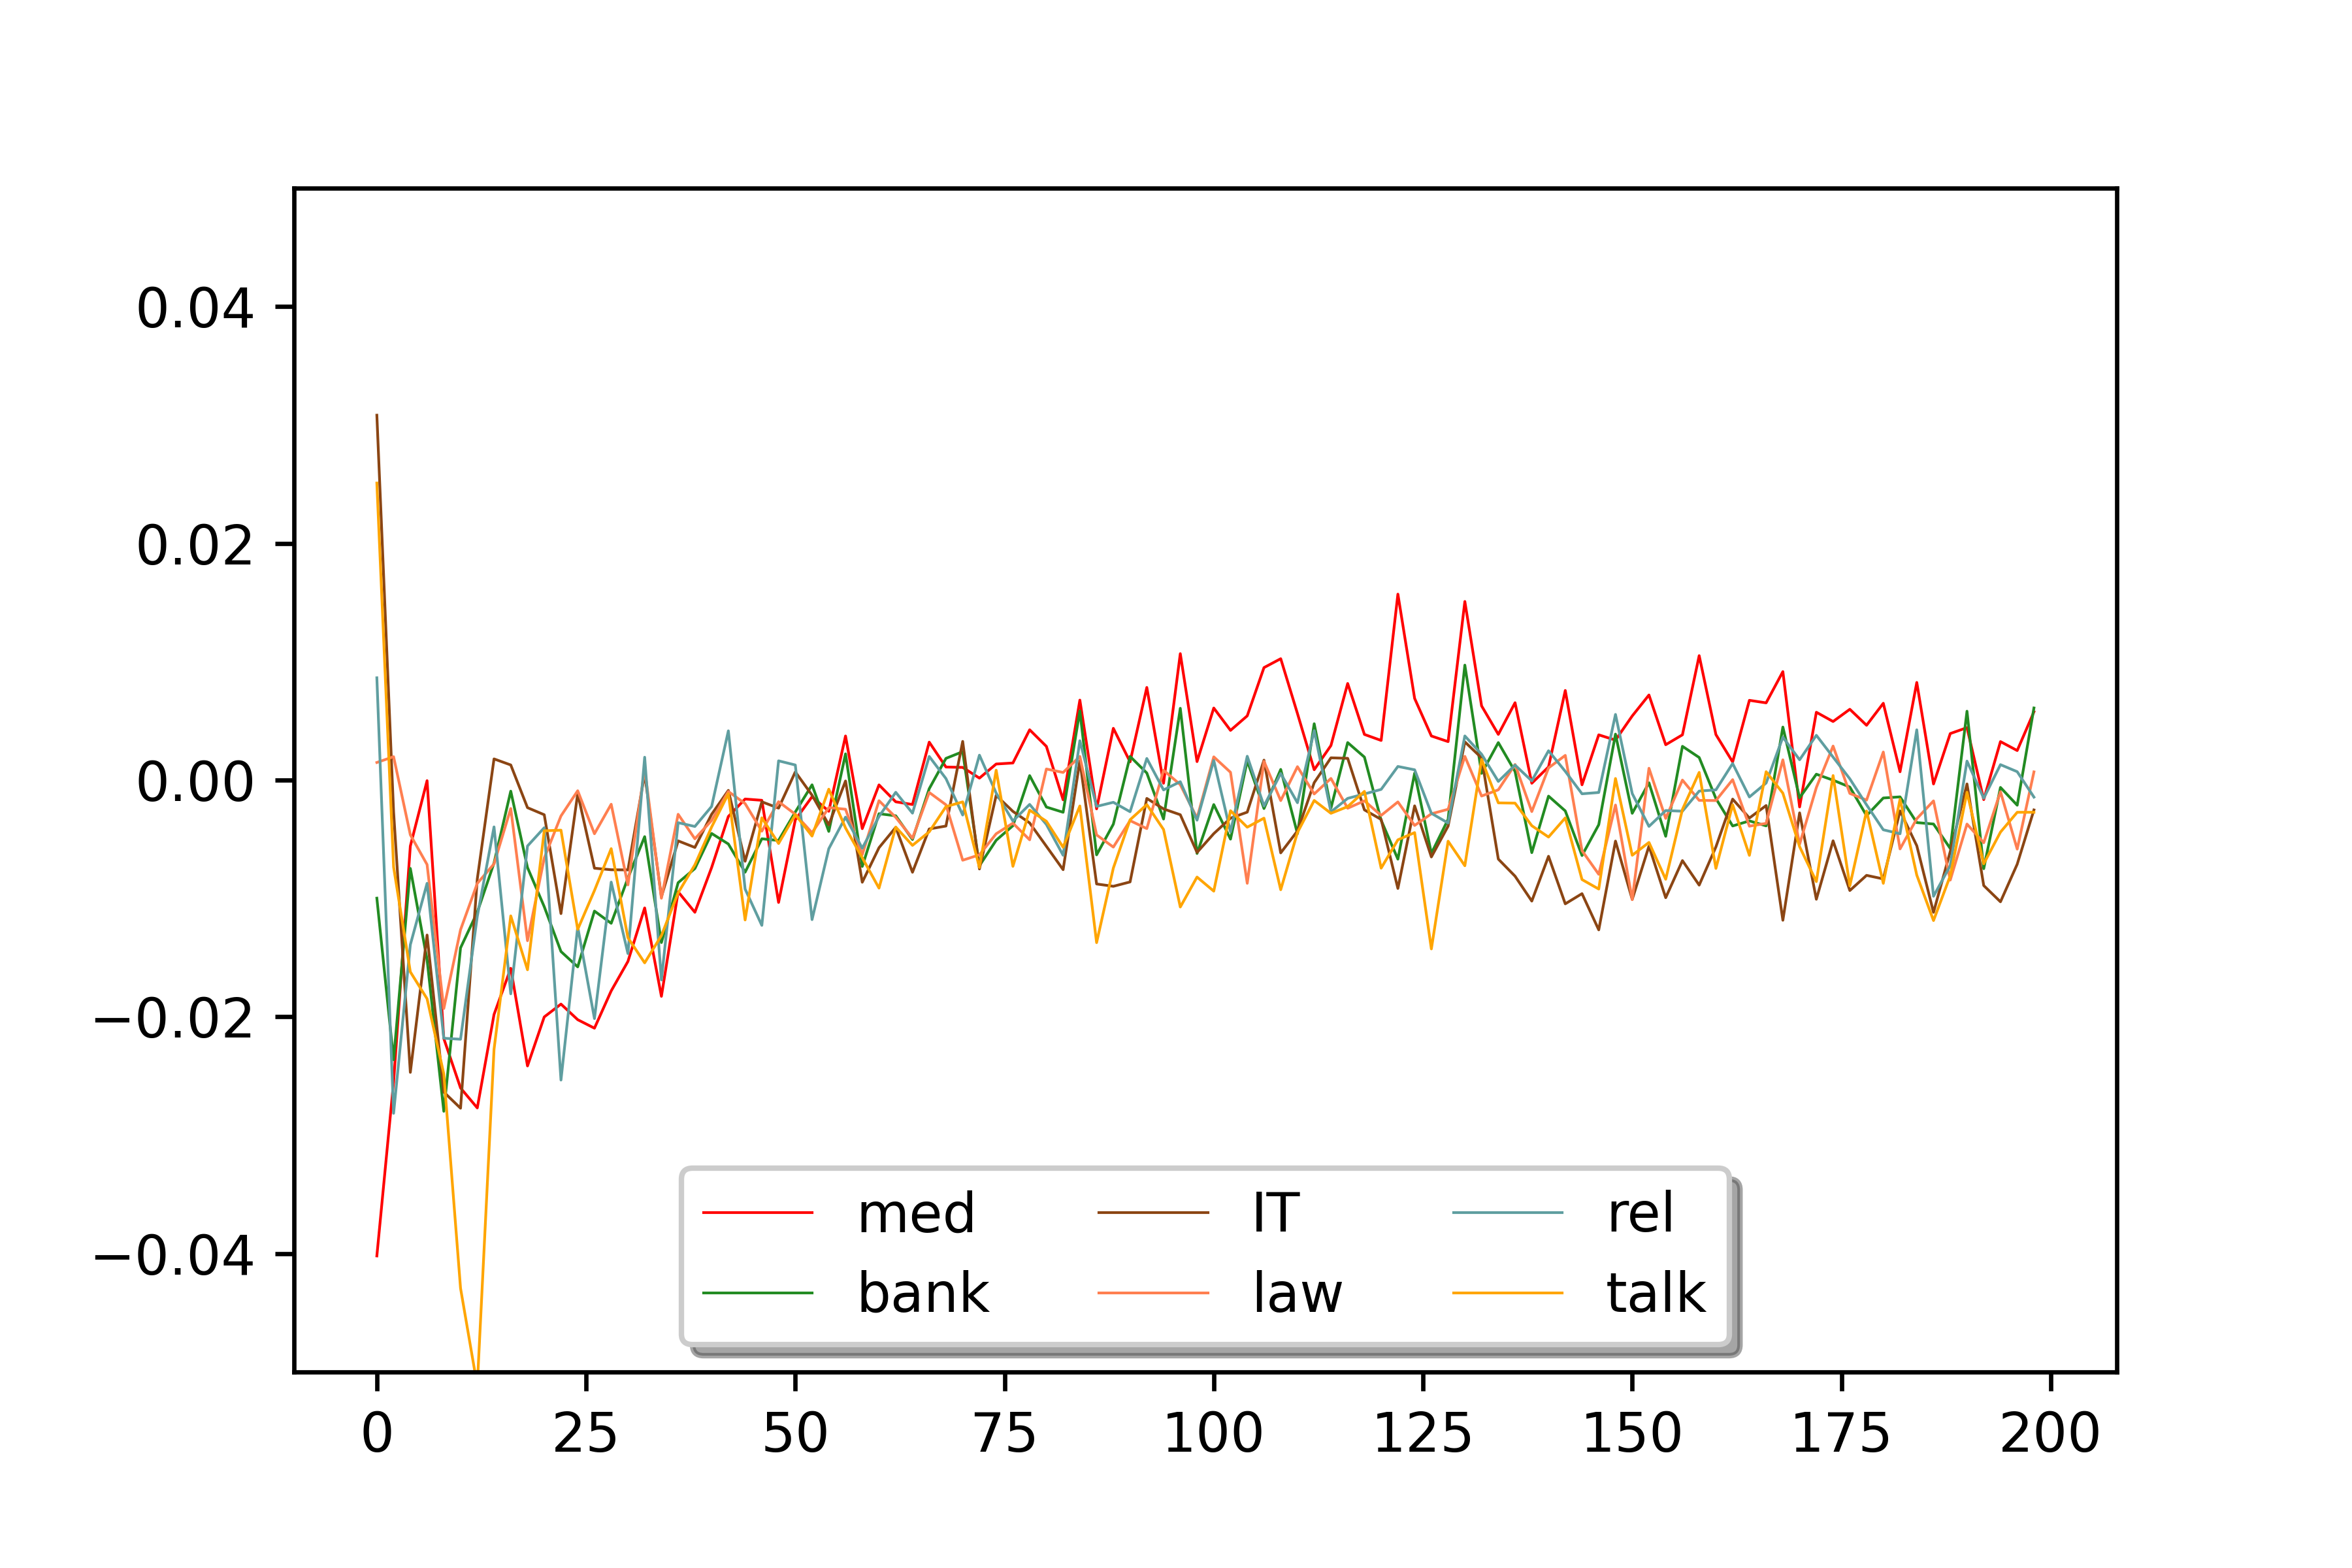
\includegraphics[width=0.97\textwidth]{graphics/rewards_loss.png}  
  \caption{MDAC}
  \label{fig:reward-loss-chap7}
\end{subfigure}
\caption{Evolution of the rewards during training.}
\label{fig:reward-chap7}
\end{figure*}

For MDAC, the magnitude of the rewards decreases dramatically from $1.e\text{-}2$ to $1.e\text{-}3$ in about first 10k iterations, then stays around $1.e\text{-}3$ until the end of the training. We have not tried to rescale the magnitude of rewards to $(\text{-}1,1)$ as proposed in \citet{Graves17automated} but left this perspective for the future work. 

For DDS, the magnitude of the rewards decreases dramatically from $1.e\text{-}1$ to $1.e\text{-}2$ in about first 10k iterations, then stays around $1.e\text{-}2$ until the end of the training.


\section{Related Work \label{sec:related-chap7}}

Most approaches to adaptive/dynamic data selection take inspiration from \citet{Bengio09curriculum}, where the notion of curriculum learning is introduced. CL relies on the notion of the ``easiness'' of a sample to schedule the presentation of training data so that the easiest examples are presented first and the hardest last. Various ways to automate CL using the framework of multi-armed bandits are explored in \citep{Graves17automated}, which has been an inspiration for our implementation. While the initial aim was primarily to improve and speed up training, CL has also proven useful for domain adaptive / multi-domain / multilingual MT, based on alternative definitions of ``easiness''.\fyDone{Ajouter Grave}
For instance, \citet{Zhang19curriculum} study supervised DA and propose a curriculum approach which progressively augments the training data: in the early stages, only in-data is used, while shards containing less relevant\footnote{Domain distance is computed with Lewis-Moore scores (based on the cross-entropy of in-domain LM and mixed-domain LM).} data are introduced in later stages. This is somehow opposite to the recommendations of \citet{Wees17dynamic}, whose \emph{gradual fine-tuning} progressively focuses on the in-domain data.

\citet{Kumar19reinforcement} use reinforcement techniques (deep Q-learning) to learn the curriculum strategy: in this work, complexity corresponds to difficulty levels which are binned using contrastive data selection. The reward is based on the decrease of the development set's loss that results from the actual data selection strategy.\fyDone{Alert: what do we do during warm-up ?} The same technique is recently applied to multilingual NMT in \citep{Kumar21learning}. \citet{Zhou20uncertainty} propose another curriculum-based approach which instead relies on \emph{instance uncertainty} as a measure of their difficulty and presents the data sample starting with the easiest (more predictable) first. Another contribution of this work is an alternative criterium for stopping the training. More related to our problems, \citet{Wang20learning-multi} adapt CL for multi-domain adaptation, where an optimal instance weighting scheme is found using Bayesian optimization techniques. Each step consists of (a) weighting instances based on relevance features, (b) fine-tuning a pretrained model using the weighted training set, and is applied iteratively to train a sequence of models. The one that maximizes the development set performance is finally retained.

\section{Conclusion and outlook}

In this study, we have presented a generic framework to perform a variety of standard adaptation tasks for machine translation, ranging from the conventional supervised domain adaptation to multi-domain adaptation and unseen domain adaptation. By experimenting with all these settings, we have shown that the same algorithm, aimed at automatically finding an effective data sampling scheme during the course of training, could be used in all these situations. This algorithm, we believe, provides us with a more sound approach to (multi-domain) DA than existing heuristics and dispenses with the costly search of optimal meta-parameters. Another contribution of our work is an experimental comparison of recent approaches to dynamic data selection. In the future, we intend to continue developing this approach and improve its effectiveness. One issue that we have left unaddressed is reward normalization. We remarked that rewards in early stages of the training have much higher magnitude than in the middle and ending stages making pre-mature judgments of the utility of each domain. \citet{Kumar19reinforcement} also reported this problem. \citet{Graves17automated} proposed a simple rule for re-scaling rewards to the interval $(-1,1)$. Another area where we need to progress is the unsupervised learning setting of Section~\ref{ssec:clda-chap7}, where our results still lag way behind that of supervised DA - this might be due to the inability of our simplistic optimization strategy to handle a large number of domains.